\part{Análisis}\label{part:analisis}
\section{Requerimientos}
\subsection{Funcionales}
\begin{itemize}
	\item La aplicación de PC deberá ser capaz de poder iniciar una conexión segura con el sistema utilizando la misma para enviar los mensajes que el cliente desee.
	\item La aplicación podrá enviar peticiones de forma de obtener el mensaje actual del cartel o incluso establecer uno nuevo. Por otra parte, también podrá pedir los datos de la red a la que el sistema estará conectado o cambiarlos.
	\item La aplicación deberá ser capaz de modificar parámetros de animación tales como frecuencia de parpadeo y velocidad de desplazamiento lateral o estaticidad.
	\item La aplicación deberá poder recuperar los valores actuales de los parámetros de animación que posee el cartel.
	\item La aplicación permitirá al usuario, ingresar por teclado el mensaje que desea mostrar mediante los caracteres que se establecen en el estándar de codificación de caracteres ISO/IEC 8859-1 (ver \cite{CodifChar}).
	\item El cartel deberá poder procesar sólo mensajes a través del protocolo diseñado específicamente para este proyecto (ver sección \ref{sec:protocolo}).
	\item El cartel deberá mostrar los mensajes que desee el usuario de forma legible.
	\item Tanto el cartel como la aplicación de PC deberán ser capaces de conectarse a una red WiFi que el cliente desee.
	\item El cartel deberá poder almacenar y modificar sus credenciales de red de forma de poder conectarse al WiFi que el cliente desee.
	\item El cartel deberá obtener una contraseña de acceso al sistema para realizar cualquier operación mencionada anteriormente.
	\item El cartel deberá mantener los datos de configuración y del mensaje que muestra, aún cuando el mismo haya sido desconectado de la red inalámbrica o de la red eléctrica.
	\item El cartel deberá poder pasar a un estado por defecto en cuanto a credenciales de red, mensaje y parámetros de animación cuando el sistema se resetea manualmente o cuando el mismo se quede en un estado incorrecto.
	\item El hardware del cartel debe poder escalar la cantidad de módulos de LEDs.
	\item El hardware del cartel debe permitir indicar la cantidad de módulos de LEDs conectados, de manera tal que el programa del microcontrolador sepa con cuántos de ellos está operando en todo momento.
	\item El sistema que controla el cartel debe estar preparado para escalar en caso de que se agreguen más módulos de LEDs.
	%TODO AMG - Requerimientos de hardware??
	\item El cartel debe tener un consumo energético bajo capaz de ser cubierto por una fuente de alimentación pequeña ($\le 1000\ \mbox{mW}$)
	\item El sistema tiene que poder ser replicado. Los componentes que lo conforman tienen que ser comercializables y obtenibles en negocios de electrónica.
	\item El cartel debe tener el tamaño suficiente para poder ser leído desde una distancia de aproximadamente 20 metros.
	\item El cartel debe poder permanecer trabajando constantemente sin alcanzar una temperatura elevada que ponga en peligro la instalación.
	\item La luminosidad de los LEDs debe ser suficientemente alta como para poder distinguirse pese a estar en ambientes iluminados artificialmente.
	\item El sistema del cartel debe ser modularizable. Esto quiere decir que pueda ser dividido en partes definidas que cumplan distintas funciones.
	\item Las dimensiones de los circuitos del cartel deben ser de un tamaño tal que no ocupen espacio adicional además del necesario para mostrar las matrices de LEDs del cartel.
	\item La longitud del cartel poder extenderse agregando módulos adicionales.
\end{itemize}

\subsection{No funcionales}
\begin{itemize}
	\item El tiempo de respuesta del cartel no debe exceder los cinco segundos.
	\item El sistema entero no debe consumir mas de 30 Watts bajo operación normal.
%	\item El sistema deberá ser capaz de aceptar sólo conexiones por TLS \cite{TLS} de forma que las conexiones y el intercambio de paquetes sea cifrado y seguro.
	%TODO AMG - Si podemos meter algunos requerimientos no funcionales más, joya!
\end{itemize}

\subsection{Interacción con el usuario}
	
	Se denomina usuario del sistema a toda persona con acceso autorizado a su configuración y puesta en marcha.	El usuario tendrá la posibilidad de agregar o quitar módulos esclavos al cartel con el fin de proveerle mayor longitud, de acceder al panel de configuración del cartel para modificar su mensaje y características del mismo.
	
	Para operar correctamente el cartel, únicamente es necesario que el usuario tenga a su disposición una PC, en la cual utilizará un aplicativo desarrollado con una interfaz gráfica para controlar el cartel. Para realizar la instalación del sistema, se requiere solamente al manual de instalación (ver \ref{sec:inst-hw}).

	No es necesario que el usuario tenga conocimientos de programación.
	Sin embargo, una noción básica de electrónica es deseable para evitar que algún componente o conexión eléctrica del sistema se vea perjudicada durante su instalación.
	
	A la hora de añadir y eliminar módulos esclavos, es necesario actualizar la información en el programa de forma de hacerle conocer al sistema, que la cantidad de módulos ha sido modificada. Esto se realiza conectando y desconectando jumpers que se encuentran en el módulo maestro del cartel.
	El usuario debe poseer un conocimiento básico de esta operación para poder realizarla satisfactoriamente.
	
	

\section{Especificaciones físicas}

	El sistema está conformado por módulos de dos tipos claramente distinguibles: un módulo maestro y módulos esclavos.

	El módulo maestro, que se caracteriza por tener la ficha de alimentación y no estar conectada a una matriz de LEDs, se encarga de controlar la cadena de módulos esclavos. Sólo un módulo de este tipo es necesario por cartel.
	Adicionalmente este componente posee un microcontrolador que gobierna la totalidad del sistema y un conjunto de jumpers que permiten establecer la cantidad de módulos esclavos con los que se operará.
	Por último esté módulo, posee un botón de reset que permite enviar al sistema a un estado conocido, ya sea ante un fallo o incluso, ante un cambio en alguno de los valores relacionados a sus credenciales de red.

	Por otro lado, están los módulos esclavos, que se encargan de controlar su matriz de LEDs para representar un mapa de bits y de funcionar como eslabón en la cadena de módulos esclavos. Se puede ver en la figura \ref{fig:dibujo-real} un dibujo ilustrativo exhibiendo los componentes más relevantes del sistema.
	\begin{description}
		\item[A: ] Fuente de alimentación (AC 220V a 5V DC).
		\item[B: ] Cables de interconexión maestro-esclavo y esclavo-esclavo.
		\item[C: ] Módulo esclavo.
		\item[D: ] Módulo maestro.
		\item[E: ] Cables de conexión a la matriz de LEDs.
		\item[F: ] Matriz de LEDs.
		\item[G: ] Pulsador de reset.
		\item[H: ] Jumpers de configuración.
		\item[I: ] NodeMCU ESP-12
		\item[J: ] MAX7219.
	\end{description}
	
	\begin{figure}[ht!]
		\begin{center}
			\centering
			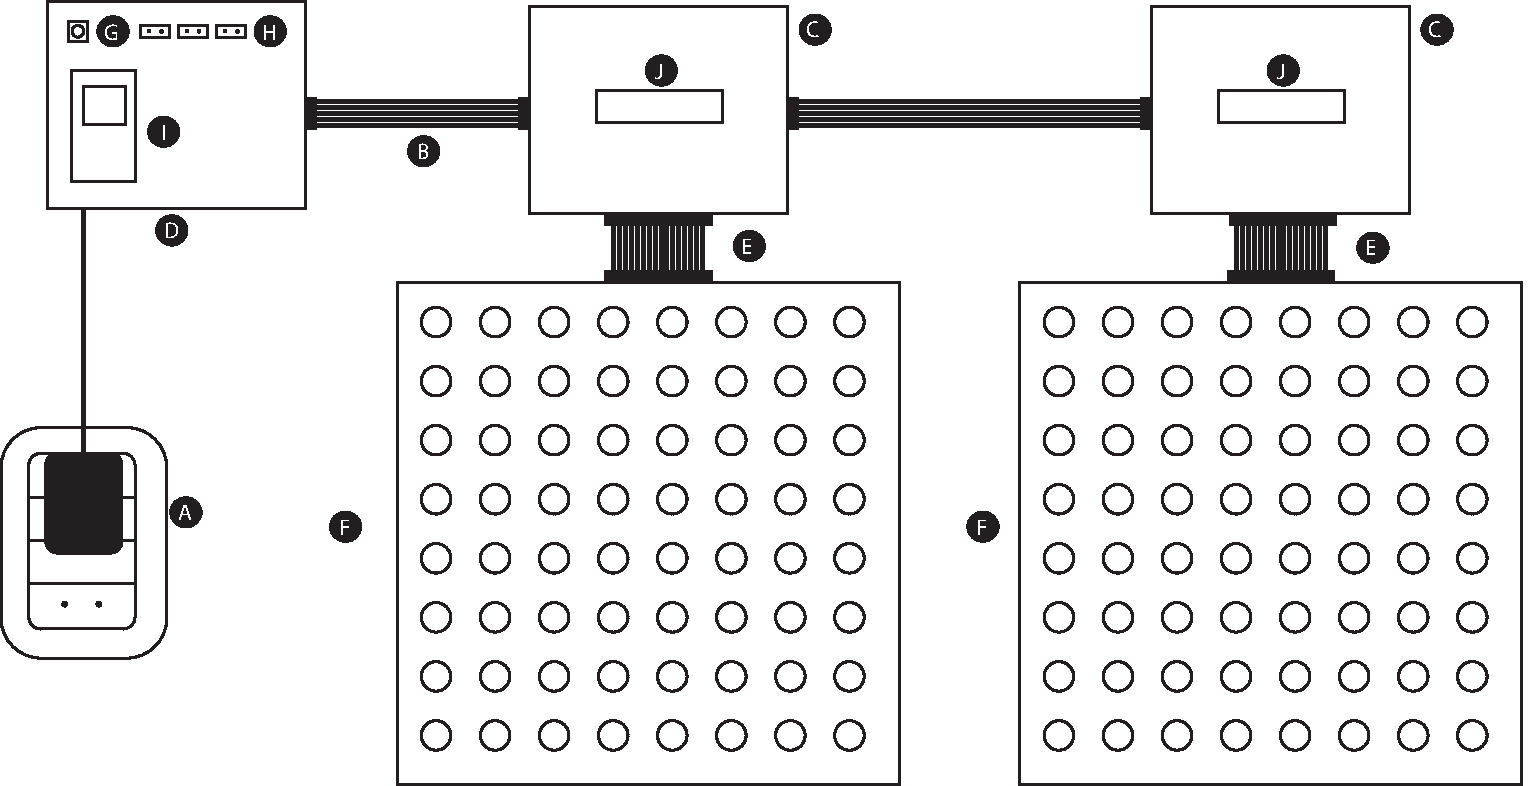
\includegraphics[width=1.1\linewidth]{imagenes/dibujo-fisico.pdf}
			\caption{Dibujo ilustrativo del hardware del sistema.}
			\label{fig:dibujo-real}
		\end{center}
	\end{figure}

	
\section{Cronograma de actividades}

En el apartado anterior del informe, se menciona la necesidad de realizar una buena planificación de las tareas a fin de obtener un panorama general respecto a la duración total del proyecto entero.

Para que el proceso de planificación arroje resultados más precisos, se recomienda dividir el sistema entero en tareas concretas e independientes y realizar una estimación de cada una de ellas de manera individual.

Un cronograma de actividades acertado, que englobe a todas las tareas requeridas para el proyecto, permite identificar la dependencia entre ellas y por consiguiente, la mejor forma para paralelizar las mismas de manera que se minimice el tiempo total de desarrollo, maximizando, a su vez, la productividad general de cada uno de los miembros del proyecto.

La otra ventaja que se percibe al realizar una planificación de las actividades que componen el sistema es que permite asignar tareas de la forma más equitativa posible a cada integrante del equipo.

Para la elaboración del cronograma de actividades del proyecto, se siguió el modelo de diagrama de Gantt que se detalla a continuación.

\subsection{Diagrama de Gantt}
El diagrama de Gantt es una eficaz herramienta para la gestión de proyectos, que permite ver, de manera gráfica, el cronograma de actividades que forman parte del programa, su duración y secuencia.

En él se muestra las etapas de las que se compone el programa diseñado y las actividades planificadas para desarrollarlo. Para ello, se señala el principio y final de cada una de estas fases por medio de diagramas de barras. De esta forma, se puede visualizar  fácilmente  el calendario global del proyecto.

\subsubsection{Pasos para elaborar un diagrama de Gantt}
Este método favorece la planificación global de proyectos. Para confeccionarlo, se deben seguir una serie de pasos necesarios, que facilitan la elaboración de este tipo de cronogramas. Los pasos se listan a continuación.

\begin{itemize}
	\item Reflejar las etapas del proyecto.
	\item Determinar las tareas principales a desarrollar.
	\item Indicar la duración de cada tarea.
	\item Señalar la interdependencia entre actividades.
	\item Establecer la lista de prioridades.
	\item Distribuir los recursos necesarios.
	\item Asignar las tareas a cada persona o equipo de trabajo.
\end{itemize}

\subsubsection{Ventajas del modelo}
Este tipo de diagramas permite visualizar el cronograma global del proyecto. 
Ésto resulta muy práctico para conocer rápidamente las fases y tareas que se llevarán a cabo, los tiempos previstos y la evolución de los mismos.

Por otra parte establece una serie de plazos realistas, que se ven reflejados en dicho esquema.
De hecho, el planteamiento de un diagrama de Gantt debe hacerse en base a fines totalmente alcanzables.
En este sentido, resulta muy útil para conseguir establecer objetivos realistas.

La elaboración del cronograma exige descomponer el proceso en diversas partes que se estructuran en pequeñas unidades. De esta forma, se establecen las fases y se detallan las acciones necesarias para llevar a cabo el sistema final. El proyecto se descompone y organiza en pequeñas metas de corta duración.

El diagrama de Gantt es una eficaz herramienta de comunicación, que permite transmitir a todos los integrantes implicados en el proyecto, la totalidad de las etapas que conforman el sistema.

\subsubsection{Desventajas del modelo}
En proyectos complejos y dinámicos puede resultar demasiado difícil su elaboración. La reorganización del cronograma puede convertirse en una tarea complicada y costosa, especialmente cuando no se dispone de las herramientas adecuadas.

Además, precisa de una evaluación y revisión continua debido a que los proyectos se vuelven dinámicos y cambiantes. Determinados imprevistos pueden modificar el cronograma entero, por lo que es necesario actualizarlo periódicamente, para que cumpla con su fin.

\subsection{Planificación de las tareas}

Para la confección del cronograma de tareas, se sigue la filosofía de diseño \emph{topdown} explicado en la sección \ref{sec:filosofia}.

En primer lugar, se deben exponer todos los requerimientos funcionales y no funcionales del proyecto entero.
En esta primera fase, se listan las funcionalidades del sistema, y sus reestricciones en cuanto a tamaño, consumo, precio.
Esta tarea, tomó lugar durante la primera semana del proyecto.

Tras haber confeccionado una lista detallada de los requerimientos que el sistema debe satisfacer, se procede a determinar los componentes necesarios para la implementación del sistema.
Entre los dispositivos más importantes para este proyecto, se encuentra el microcontrolador a utilizar y los drivers de LEDs.
Para el primero se asignó dos semanas de estudio de las diferentes alternativas en la industria debido a la gran variedad de microcontroladores que existe. Mientras que para los drivers, se asignó solo una semana.

En paralelo con la elección de los componentes, se decide realizar el modelo de la solución general del sistema del lado del software, al cual se le asignó dos semanas. Esta etapa incluye tanto la investigación de las tecnologías de desarrollo compatibles con los distintos microcontroladores de la industria, así como también, la elección del lenguaje de programación, frameworks, confeccionado de UMLs y diagramas de estados.

Tras elegir los componentes de hardware que se utilizarán en el desarrollo del sistema, se procede a armar el conexionado inicial del cartel , analizando las interfaces de comunicación entre los distintos dispositivos electrónicos, en conjunto con los valores de tensión a los que trabajan.
En particular, se hace un especial hincapié en la interconexión entre el microcontrolador y los drivers de LEDs.
Para esta tarea se asignó una semana de investigación y otra más para el desarrollo del prototipo del cartel sobre una protoboard. Esto abarca el prototipado de un esclavo y de un maestro.

En paralelo con esta última tarea, se procede a realizar el diseño del protocolo de comunicación de red entre la aplicación de PC y el firmware del microcontrolador. Para este punto, es necesario tener en claro todas las funciones que puede realizar el sistema ya que las mismas van a convertirse en comandos que se intercambiarán entre los dos módulos de software mencionados. Para el diseño e implementación de esta tarea, se asignaron tres semanas de desarrollo.

En conjunto con la codificación del protocolo de comunicación de red, se procedió a realizar el diseño del esquemático y posteriormente el diseño de la PCB. Para la realización de esta tarea, se estimó tres semanas de trabajo puesto que incluye tanto el diseño del maestro como del esclavo.

Al finalizar el proceso de implementación del protocolo, se decidió a realizar en paralelo el desarrollo de la aplicación de PC y del firmware del microcontrolador. Para cada tarea se asignó dos y tres semanas respectivamente.

Luego de completada esta última fase, se procede a la utilización del protocolo de red TLS, para brindar cifrado, autenticación e integridad a las conexiones de red que se establecen entre la aplicación de PC y el firmware del microcontrolador.

Tras concluir con las dos aplicaciones de software, se destinaron dos semanas a la prueba en conjunto de estas dos componentes.

Por otra parte, siguiendo con el cronograma y finalizada la etapa anterior, la semana 9 a la 11, se destinó a la fabricación del los PCBs. Dicha etapa se detalla en la sección \ref{sec:fab-PCB}. Cabe recordar que esta tarea incluye la confección del maestro y de dos esclavos.

Luego, se estimaron dos semanas adicionales para el proceso de soldado de los componentes sobre la plaqueta y el testeo de conductividad eléctrica entre los módulos de hardware.

Finalmente, tras haber realizado la prueba general del software, se destina la última semana de producción para las pruebas generales donde se evalúa la interacción de los programas con el cartel propiamente dicho.

La figura \ref{fig:cronograma} se observa en detalle el tiempo empleado en cada etapa.

\begin{figure}[ht!]
	\begin{center}
		\centering
		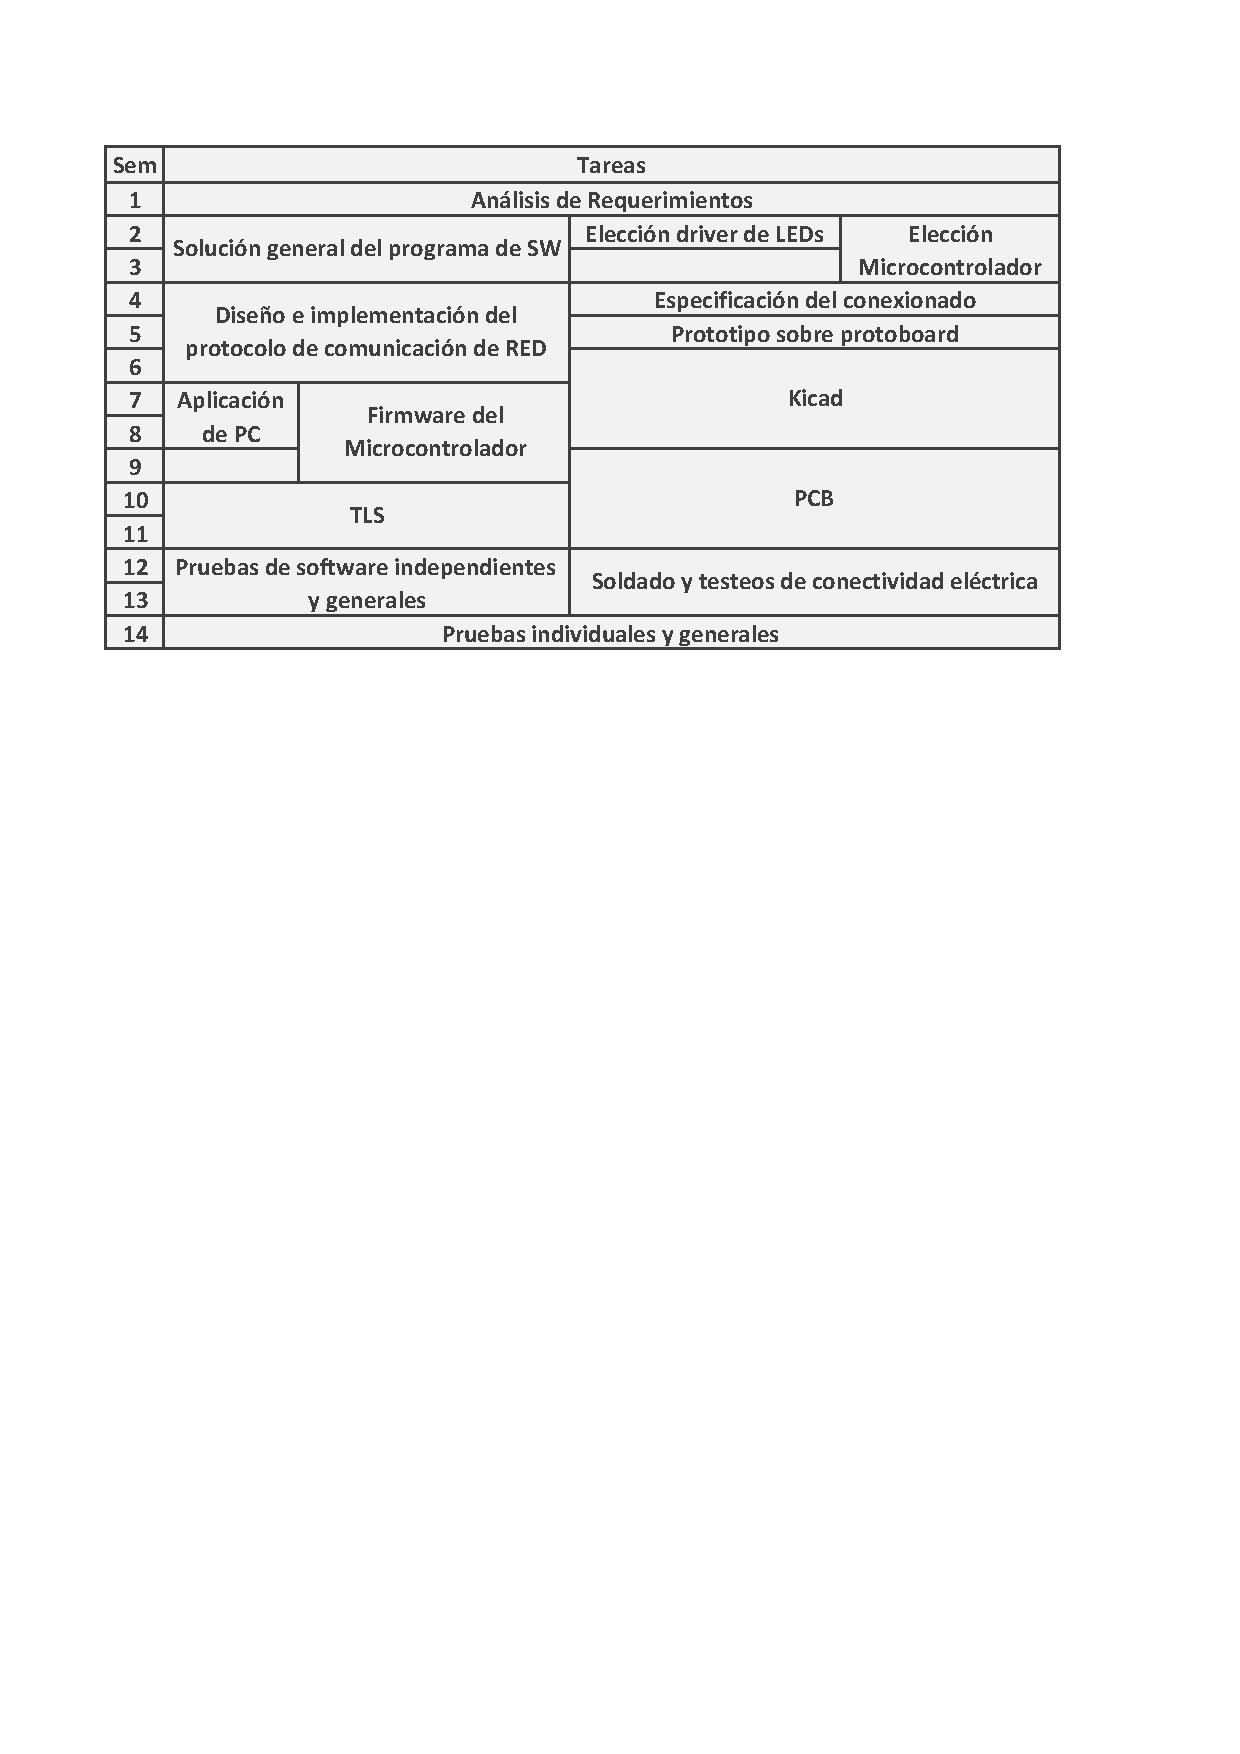
\includegraphics[width=\linewidth]{tablas/cronograma-v2.pdf}
		\caption{Coronograma final del proyecto.}
		\label{fig:cronograma}
	\end{center}
\end{figure}

\section{Componentes de hardware}
A la hora de construir el cartel, se debe armar tanto un módulo maestro y uno o más módulos esclavos, siendo éstos últimos los encargados de mostrar los mensajes en el cartel.
En el apéndice \ref{sec:materiales} se listan los componentes de cada módulo y las herramientas necesarias para la construcción de los mismos.


\section{Estimación de costos}
Como se explicó en la sección anterior, en todo proyecto es necesario realizar tanto una estimación del tiempo de desarrollo del sistema como una aproximación a los costos que tendrá el mismo.
Por dicho motivo, en el apéndice \ref{sec:presupuesto} se detalla el valor aproximado que posee cada material listado previamente.